\section{Training for DUMs}
\label{sec:training}

In this section, we study the importance of the training procedure in the performance of DUMs. To this end, we look at \emph{decoupling the learning rates} of the core encoder architecture and the uncertainty head, different \emph{training schemes}, and different \emph{pretraining schemes}.

\textbf{Decoupling learning rates.} We decouple the learning rates of the core architecture and the uncertainty head. We show the validation results for CIFAR100 as ID and SVHN as OOD with the core architecture ResNet18 in \cref{fig:decoupled_test}.
\underline{\textit{Observation:}} We observe that, when using different learning rates for the core architecture and the uncertainty head, NatPN improves Brier Score and OOD epistemic results and DUE significantly improves both predictive and uncertainty results. Hence, this shows that decoupling learning rates can improve results of DUMs, thus suggesting that the core architecture and the uncertainty head have training dynamics which requires different considerations.

\begin{figure}[!htb]
    \centering
    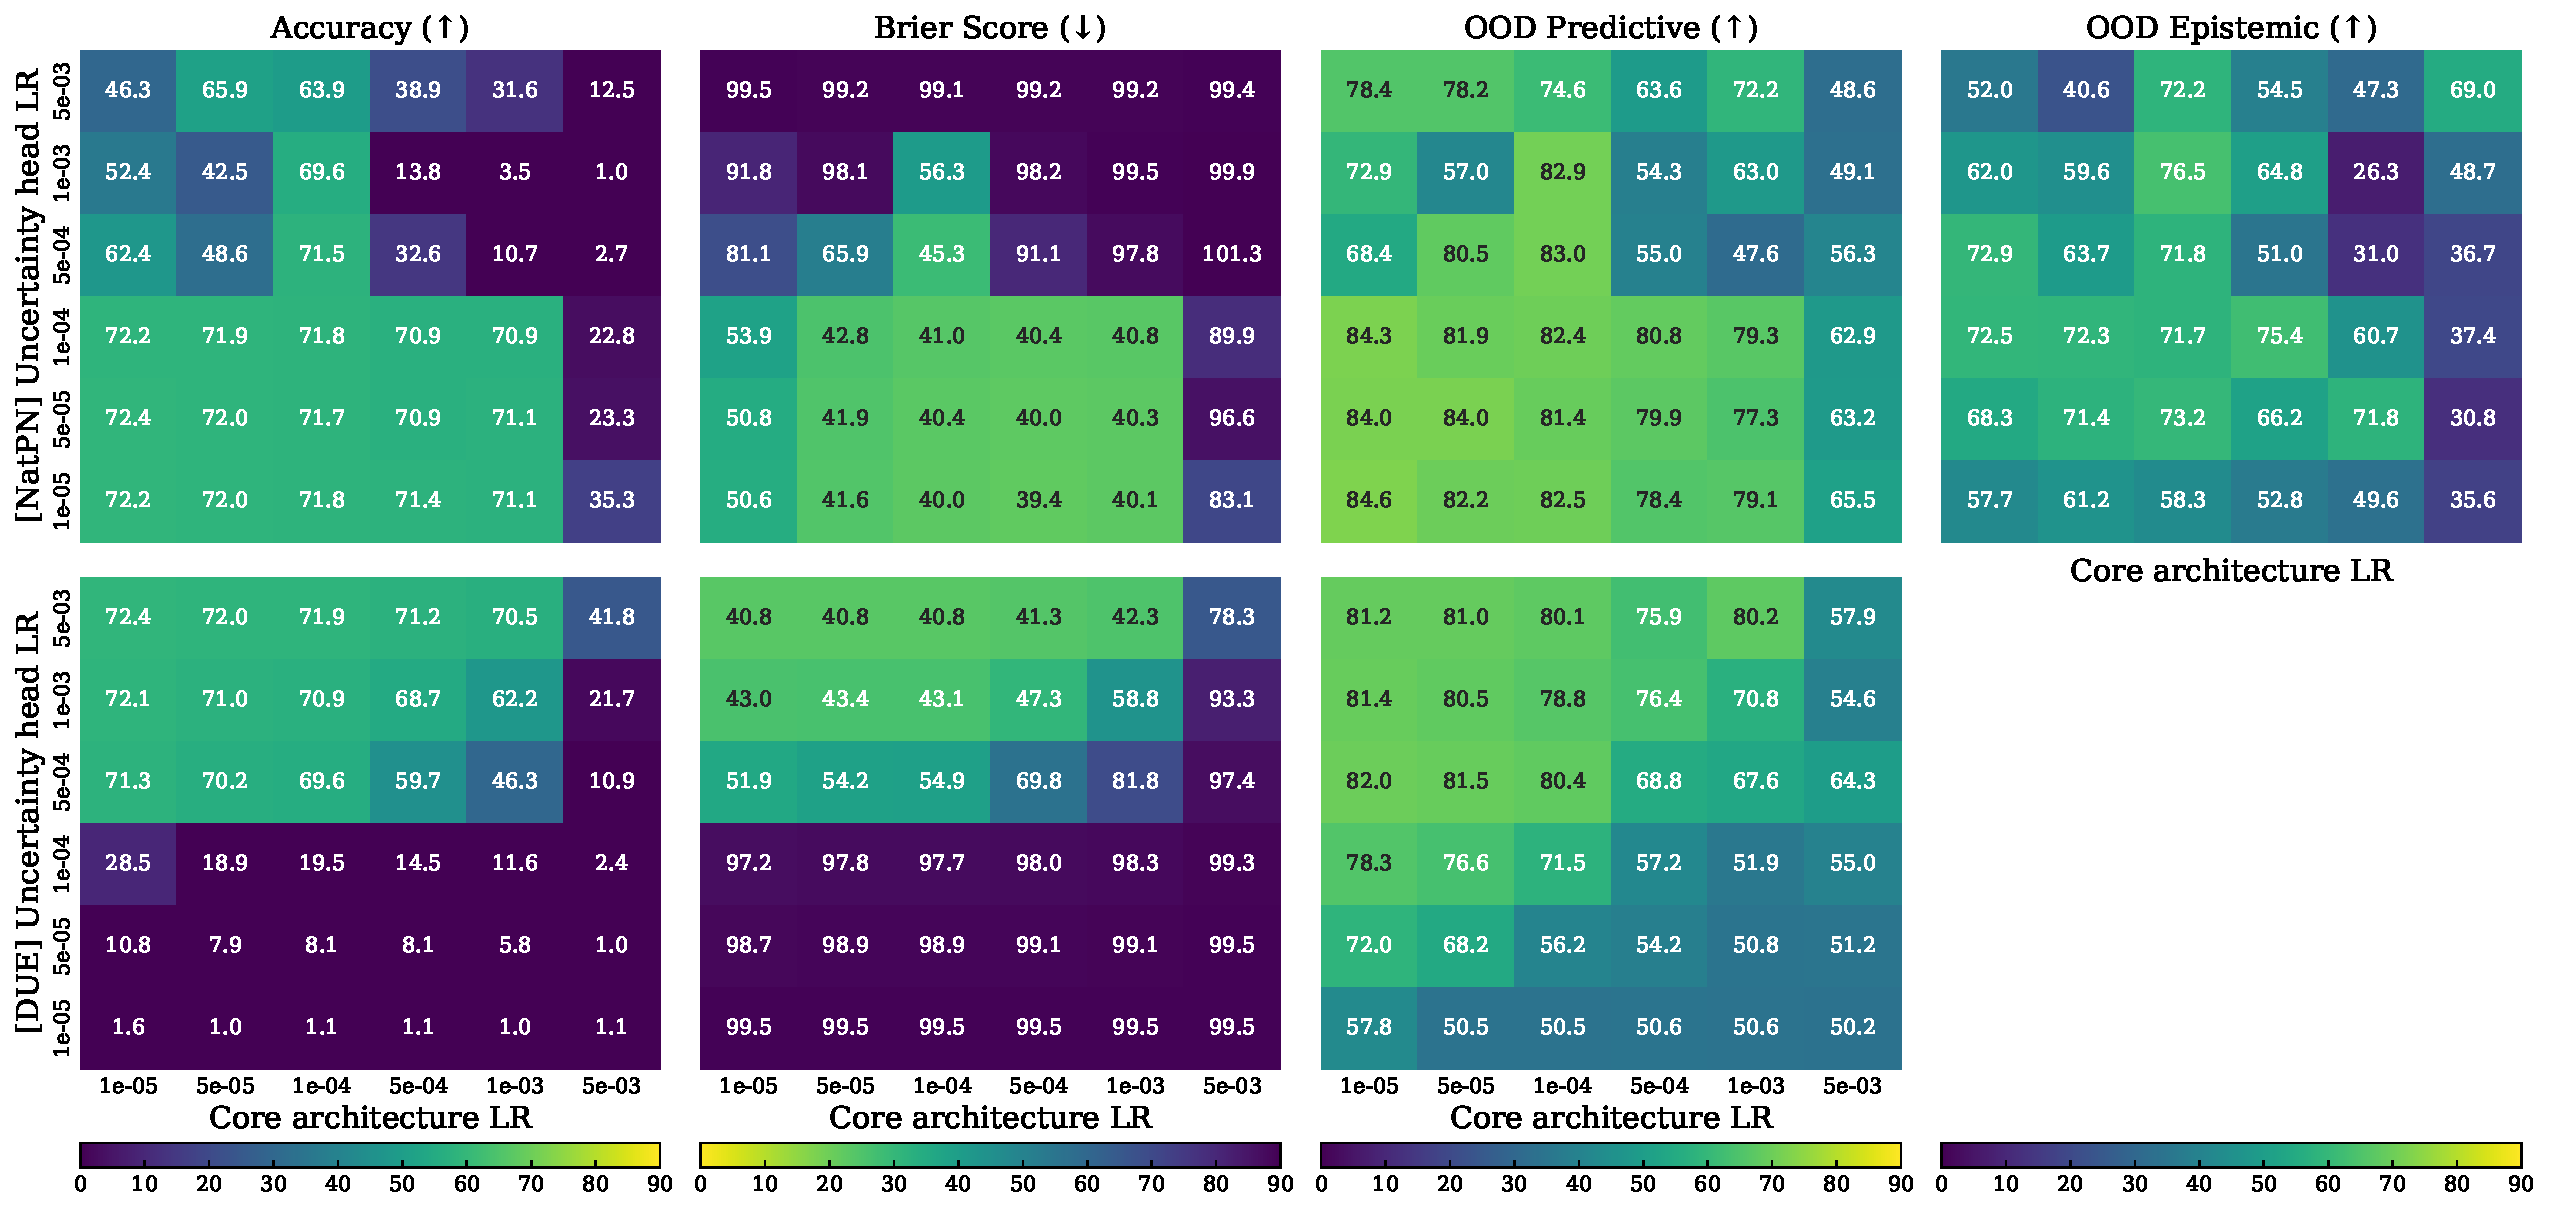
\includegraphics[width=0.8\linewidth]{sections/008_iclr2023/figures/decoupled_test.pdf}
    \caption{Results of DUMS on CIFAR100 with ResNet18 when \textbf{decoupling learning rates} of the core architecture and the uncertainty head. Decoupling learning rates improve DUMs performance. }
    \label{fig:decoupled_test}
\end{figure}

\textbf{Training schemes.} We compare two settings: the \textit{joint} training in which we jointly train the weights of the core architecture and uncertainty head, and the \textit{sequential} training in which we only train the uncertainty head by keeping the weights of the pretrained core architecture fixed. For each of the setting, we apply two additional techniques to stabilize the training: adding a \textit{batch normalization} to the last layer of the encoder to enforce latent representations to locate in a normalized region \citep{ioffe2015bn,NatPN2021}, and \textit{resetting the last layer} to retrain its weights to improve robustness to spurious correlation \citep{kirichenko2022reset}. We show the results for CIFAR100 as ID and five difference OOD datasets with the ResNet18 as core architecture in \cref{tab:training_schema} and additional results in the appendix \cref{tab:training_schema_ood}.
\underline{\textit{Observation:}} We observe that, compared to its sequential counterpart, joint training consistently improves DUMs performance for most metrics, thus suggesting that joint training should be preferred in practice for DUMs. Furthermore, while the GP-based method DUE does not benefit from stabilization techniques, we observe that they can significantly increase performance of the density-based method NatPN. This behavior is intuitively explained by the practical difficulty to accurately fit densities in high dimensional latent space. This can be significantly improved by using more powerful density estimator (see \cref{tab:normalizing_flow} in appendix).

\textbf{Pretraining schemes.} We compare multiple training schemes which differ in terms of \emph{amount} and \emph{quality} of data used for pretraining. Hence, we do not pretrain the core architecture or pretrain it with 10\% of CIFAR100, 100\% of CIFAR100 without and with Gaussian noise, or ImageNet. We show the results for CIFAR100 as ID and five different OOD datasets with ResNet50 as core architecture in \cref{tab:training_pretrain} and additional results in the appendix \cref{tab:training_pretrain_ood}.
\underline{\textit{Observation:}} We observe that, while too few data for pretraining does not improve final performance of DUMs, the overall performance significantly increase when the encoder is pretrained with high quantity and high quality of data.  Similarly to \citet{why-nf-fail-ood}, this suggests that the embedding quality is important to improve uncertainty quantification. Here, we show additionally that embeddings pretrained with many high quality data are crucial to facilitate the prediction of the uncertainty head.

\begin{table}[!htp]\centering
    \caption{Results of DUMs on CIFAR100 with ResNet18 under different \textbf{training schemes} using \textit{joint/sequential} training with no additional layer, an additional batch norm layer, or resetting the last layer. Gray cells indicate the best between \textit{joint/sequential} while bold numbers indicate the best overall. OOD results are averaged over OOD datasets. We observe that joint training works best and stabilization techniques can improve performances.}
    \label{tab:training_schema}
    \tiny
    
    \resizebox{0.9\textwidth}{!}{%
    \begin{tabular}{llccccc}
        \toprule
        \textbf{Method} &\textbf{Train Schema} &\textbf{Accuracy ($\uparrow$)} &\textbf{Brier Score ($\downarrow$)} &\textbf{OOD Pred. ($\uparrow$)} &\textbf{OOD Epis. ($\uparrow$)} \\
        \midrule
        \multirow{6}{*}{NatPN} 
        & joint &71.12 $\pm$ 0.18 & \cellcolor{mycolor}41.06 $\pm$ 0.18 & \cellcolor{mycolor}75.17 $\pm$ 1.60 & \cellcolor{mycolor}63.94 $\pm$ 2.80 \\
        & joint + bn &71.60 $\pm$ 0.14 &\cellcolor{mycolor}41.11 $\pm$ 0.12 & 74.22 $\pm$ 0.94 & \cellcolor{mycolor}66.17 $\pm$ 2.55 \\
        & joint + reset &71.61 $\pm$ 0.18 & \cellcolor{mycolor}\textbf{40.76 $\pm$ 0.18} &\cellcolor{mycolor}\textbf{75.35 $\pm$ 0.71} & \cellcolor{mycolor}\textbf{69.02 $\pm$ 1.49} \\
        % \cmidrule[0.1pt](lr){2-6}
        & sequential & \cellcolor{mycolor}\textbf{72.00 $\pm$ 0.19} &42.20 $\pm$ 0.09 &75.09 $\pm$ 0.86 &53.49 $\pm$ 2.56 \\
        & sequential + bn & \cellcolor{mycolor}71.98 $\pm$ 0.18 & 42.39 $\pm$ 0.11 & \cellcolor{mycolor}75.01 $\pm$ 0.86 &52.34 $\pm$ 2.81 \\
        & sequential + reset & \cellcolor{mycolor}71.79 $\pm$ 0.17 &40.95 $\pm$ 0.14 &74.63 $\pm$ 0.85 &61.90 $\pm$ 2.14 \\
        \midrule
        \multirow{6}{*}{DUE} 
        & joint & \cellcolor{mycolor}\textbf{72.33 $\pm$ 0.11} & \cellcolor{mycolor}\textbf{40.80 $\pm$ 0.11} &74.74 $\pm$ 0.89 &- \\
        & joint + bn & \cellcolor{mycolor}72.30 $\pm$ 0.09 & \cellcolor{mycolor}40.85 $\pm$ 0.12 &74.63 $\pm$ 0.95 &- \\
        & joint + reset & \cellcolor{mycolor}71.94 $\pm$ 0.12 & \cellcolor{mycolor}41.43 $\pm$ 0.12 &74.89 $\pm$ 0.76 &- \\
        % \cmidrule[0.1pt](lr){2-6}
        & sequential &72.07 $\pm$ 0.10 &41.66 $\pm$ 0.10 & \cellcolor{mycolor}74.82 $\pm$ 0.90 &- \\
        & sequential + bn &72.04 $\pm$ 0.13 &41.73 $\pm$ 0.11 & \cellcolor{mycolor}74.88 $\pm$ 0.95 &- \\
        & sequential + reset &71.56 $\pm$ 0.14 &42.30 $\pm$ 0.11 & \cellcolor{mycolor}\textbf{75.08 $\pm$ 1.01} &- \\
        \bottomrule
    \end{tabular}
    }
\end{table}

\begin{table}[!htp]\centering
    \caption{Results of DUMs with ResNet50 under different \textbf{pretraining schemes} using no pretraining, pretraining on 10\% of CIFAR100, 100\% of CIFAR100 without Gaussian noise and with Gaussian noise, or ImageNet. OOD results are averaged over OOD datasets. Bold numbers indicate best results among all settings. We observe that high quantity and high quality of data can improve performances.}
    \label{tab:training_pretrain}
    \tiny
    
    \resizebox{0.9\textwidth}{!}{%
    \begin{tabular}{llccccc}\toprule
        \textbf{Method} &\textbf{Pretrain Schema} &\textbf{Accuracy ($\uparrow$)} &\textbf{Brier Score ($\downarrow$)} &\textbf{OOD Pred. ($\uparrow$)} &\textbf{OOD Epis. ($\uparrow$)} \\
        \midrule
        \multirow{6}{*}{NatPN} &None &78.45 $\pm$ 1.94 &30.16 $\pm$ 2.57 &79.85 $\pm$ 3.30 &85.81 $\pm$ 2.05 \\
        &C100 (10\%) &67.25 $\pm$ 0.71 &44.69 $\pm$ 0.94 &68.10 $\pm$ 1.90 &78.50 $\pm$ 3.27 \\
        &C100 (100\%) + $\gN(0.5)$ &72.50 $\pm$ 1.07 &39.36 $\pm$ 1.43 &68.66 $\pm$ 3.76 &73.54 $\pm$ 1.84 \\
        &C100 (100\%) + $\gN(0.1)$ &75.25 $\pm$ 0.61 &35.99 $\pm$ 0.88 &69.78 $\pm$ 4.65 &75.81 $\pm$ 2.85 \\
        &C100 (100\%) &76.31 $\pm$ 0.45 &34.32 $\pm$ 0.51 &78.95 $\pm$ 3.19 &76.91 $\pm$ 2.64 \\
        &ImageNet &\textbf{84.22 $\pm$ 0.12} &\textbf{23.67 $\pm$ 0.27} &\textbf{84.95 $\pm$ 1.48} &\textbf{89.08 $\pm$ 0.70} \\
        \midrule
        \multirow{6}{*}{DUE} &None &72.41 $\pm$ 0.24 &47.35 $\pm$ 0.25 &80.04 $\pm$ 1.28 &- \\
        &C100 (10\%) &63.86 $\pm$ 0.58 &50.94 $\pm$ 0.53 &72.44 $\pm$ 1.32 &- \\
        &C100 (100\%) &76.38 $\pm$ 0.35 &36.89 $\pm$ 0.50 &81.71 $\pm$ 1.87 &- \\
        &C100 (100\%) + $\gN(0.5)$ &72.10 $\pm$ 1.00 &42.48 $\pm$ 1.18 &74.89 $\pm$ 1.97 &- \\
        &C100 (100\%) + $\gN(0.1)$ &75.31 $\pm$ 0.91 &38.31 $\pm$ 1.22 &79.43 $\pm$ 1.93 &- \\
        &ImageNet &\textbf{82.42 $\pm$ 0.14} &\textbf{28.09 $\pm$ 0.19} &\textbf{90.24 $\pm$ 0.51} &- \\
        \bottomrule
        \end{tabular}
    }
\end{table}






% \begin{table}[!htb]
% \centering
% \tiny

% \begin{minipage}[t]{0.48\textwidth}
% \caption{Results of DUMs on CIFAR100 with ResNet18 under different \textbf{training schemes} using \textit{joint/sequential} training with no additional layer, an additional batch norm layer, or resetting the last layer. Gray cells indicate the best between \textit{joint/sequential} while bold numbers indicate the best overall. OOD results are averaged over OOD datasets. We observe that joint training works best and stabilization techniques can improve performances.}
% \label{tab:training_schema}
% \resizebox{\textwidth}{!}{%
% \begin{tabular}{llccccc}
% \toprule
% \textbf{Method} &\textbf{Train Schema} &\textbf{Accuracy ($\uparrow$)} &\textbf{Brier Score ($\downarrow$)} &\textbf{OOD Pred. ($\uparrow$)} &\textbf{OOD Epis. ($\uparrow$)} \\
% \midrule
% \multirow{6}{*}{NatPN} 
% & joint &71.12 $\pm$ 0.18 & \cellcolor{mycolor}41.06 $\pm$ 0.18 & \cellcolor{mycolor}75.17 $\pm$ 1.60 & \cellcolor{mycolor}63.94 $\pm$ 2.80 \\
% & joint + bn &71.60 $\pm$ 0.14 &\cellcolor{mycolor}41.11 $\pm$ 0.12 & 74.22 $\pm$ 0.94 & \cellcolor{mycolor}66.17 $\pm$ 2.55 \\
% & joint + reset &71.61 $\pm$ 0.18 & \cellcolor{mycolor}\textbf{40.76 $\pm$ 0.18} &\cellcolor{mycolor}\textbf{75.35 $\pm$ 0.71} & \cellcolor{mycolor}\textbf{69.02 $\pm$ 1.49} \\
% % \cmidrule[0.1pt](lr){2-6}
% & sequential & \cellcolor{mycolor}\textbf{72.00 $\pm$ 0.19} &42.20 $\pm$ 0.09 &75.09 $\pm$ 0.86 &53.49 $\pm$ 2.56 \\
% & sequential + bn & \cellcolor{mycolor}71.98 $\pm$ 0.18 & 42.39 $\pm$ 0.11 & \cellcolor{mycolor}75.01 $\pm$ 0.86 &52.34 $\pm$ 2.81 \\
% & sequential + reset & \cellcolor{mycolor}71.79 $\pm$ 0.17 &40.95 $\pm$ 0.14 &74.63 $\pm$ 0.85 &61.90 $\pm$ 2.14 \\
% \midrule
% \multirow{6}{*}{DUE} 
% & joint & \cellcolor{mycolor}\textbf{72.33 $\pm$ 0.11} & \cellcolor{mycolor}\textbf{40.80 $\pm$ 0.11} &74.74 $\pm$ 0.89 &- \\
% & joint + bn & \cellcolor{mycolor}72.30 $\pm$ 0.09 & \cellcolor{mycolor}40.85 $\pm$ 0.12 &74.63 $\pm$ 0.95 &- \\
% & joint + reset & \cellcolor{mycolor}71.94 $\pm$ 0.12 & \cellcolor{mycolor}41.43 $\pm$ 0.12 &74.89 $\pm$ 0.76 &- \\
% % \cmidrule[0.1pt](lr){2-6}
% & sequential &72.07 $\pm$ 0.10 &41.66 $\pm$ 0.10 & \cellcolor{mycolor}74.82 $\pm$ 0.90 &- \\
% & sequential + bn &72.04 $\pm$ 0.13 &41.73 $\pm$ 0.11 & \cellcolor{mycolor}74.88 $\pm$ 0.95 &- \\
% & sequential + reset &71.56 $\pm$ 0.14 &42.30 $\pm$ 0.11 & \cellcolor{mycolor}\textbf{75.08 $\pm$ 1.01} &- \\
% \bottomrule
% \end{tabular}
% }\end{minipage}\quad%
% %
% %
% \begin{minipage}[t]{0.48\textwidth}
% \caption{Results of DUMs with ResNet50 under different \textbf{pretraining schemes} using no pretraining, pretraining on 10\% of CIFAR100, 100\% of CIFAR100 without Gaussian noise and with Gaussian noise, or ImageNet. OOD results are averaged over OOD datasets. Bold numbers indicate best results among all settings. We observe that high quantity and high quality of data can improve performances.}
% \label{tab:training_pretrain}

% \resizebox{\textwidth}{!}{%
% \begin{tabular}{llccccc}\toprule
% \textbf{Method} &\textbf{Pretrain Schema} &\textbf{Accuracy ($\uparrow$)} &\textbf{Brier Score ($\downarrow$)} &\textbf{OOD Pred. ($\uparrow$)} &\textbf{OOD Epis. ($\uparrow$)} \\
% \midrule
% \multirow{6}{*}{NatPN} &None &78.45 $\pm$ 1.94 &30.16 $\pm$ 2.57 &79.85 $\pm$ 3.30 &85.81 $\pm$ 2.05 \\
% &C100 (10\%) &67.25 $\pm$ 0.71 &44.69 $\pm$ 0.94 &68.10 $\pm$ 1.90 &78.50 $\pm$ 3.27 \\
% &C100 (100\%) + $\gN(0.5)$ &72.50 $\pm$ 1.07 &39.36 $\pm$ 1.43 &68.66 $\pm$ 3.76 &73.54 $\pm$ 1.84 \\
% &C100 (100\%) + $\gN(0.1)$ &75.25 $\pm$ 0.61 &35.99 $\pm$ 0.88 &69.78 $\pm$ 4.65 &75.81 $\pm$ 2.85 \\
% &C100 (100\%) &76.31 $\pm$ 0.45 &34.32 $\pm$ 0.51 &78.95 $\pm$ 3.19 &76.91 $\pm$ 2.64 \\
% &ImageNet &\textbf{84.22 $\pm$ 0.12} &\textbf{23.67 $\pm$ 0.27} &\textbf{84.95 $\pm$ 1.48} &\textbf{89.08 $\pm$ 0.70} \\
% \midrule
% \multirow{6}{*}{DUE} &None &72.41 $\pm$ 0.24 &47.35 $\pm$ 0.25 &80.04 $\pm$ 1.28 &- \\
% &C100 (10\%) &63.86 $\pm$ 0.58 &50.94 $\pm$ 0.53 &72.44 $\pm$ 1.32 &- \\
% &C100 (100\%) &76.38 $\pm$ 0.35 &36.89 $\pm$ 0.50 &81.71 $\pm$ 1.87 &- \\
% &C100 (100\%) + $\gN(0.5)$ &72.10 $\pm$ 1.00 &42.48 $\pm$ 1.18 &74.89 $\pm$ 1.97 &- \\
% &C100 (100\%) + $\gN(0.1)$ &75.31 $\pm$ 0.91 &38.31 $\pm$ 1.22 &79.43 $\pm$ 1.93 &- \\
% &ImageNet &\textbf{82.42 $\pm$ 0.14} &\textbf{28.09 $\pm$ 0.19} &\textbf{90.24 $\pm$ 0.51} &- \\
% \bottomrule
% \end{tabular}
% }\end{minipage}
% \end{table}

% \begin{table}[!htp]\centering
% \caption{\textbf{Pretrain schema.} Both DUMs benefits from the quantity of data under the ImageNet pretrained encoder. The reported OOD results are an average over all the independent OOD dataset result. The encoder ResNet50 from torchvision is used for the schemas.}
% \label{tab:training_pretrain}
% \tiny
% \begin{tabular}{llccccc}\toprule
% \textbf{Model} &\textbf{Pretrain Schema} &\textbf{Accuracy} &\textbf{Brier Score} &\textbf{OOD Pred.} &\textbf{OOD Epis.} \\
% \midrule
% \multirow{4}{*}{NatPN} &None &78.45 $\pm$ 1.94 &30.16 $\pm$ 2.57 &79.85 $\pm$ 3.30 &85.81 $\pm$ 2.05 \\
% &C100 (10\%) &67.25 $\pm$ 0.71 &44.69 $\pm$ 0.94 &68.10 $\pm$ 1.90 &78.50 $\pm$ 3.27 \\
% &C100 (100\%) &76.31 $\pm$ 0.45 &34.32 $\pm$ 0.51 &78.95 $\pm$ 3.19 &76.91 $\pm$ 2.64 \\
% &\textbf{ImageNet} &\textbf{84.22 $\pm$ 0.12} &\textbf{23.67 $\pm$ 0.27} &\textbf{84.95 $\pm$ 1.48} &\textbf{89.08 $\pm$ 0.70} \\
% \midrule
% \multirow{4}{*}{DUE} &None &72.41 $\pm$ 0.24 &47.35 $\pm$ 0.25 &80.04 $\pm$ 1.28 &- \\
% &C100 (10\%) &63.86 $\pm$ 0.58 &50.94 $\pm$ 0.53 &72.44 $\pm$ 1.32 &- \\
% &C100 (100\%) &76.38 $\pm$ 0.35 &36.89 $\pm$ 0.50 &81.71 $\pm$ 1.87 &- \\
% &\textbf{ImageNet} &\textbf{82.42 $\pm$ 0.14} &\textbf{28.09 $\pm$ 0.19} &\textbf{90.24 $\pm$ 0.51} &- \\
% \bottomrule
% \end{tabular}
% \end{table}
